
\section{Muon system}

%%%%%% SLIDE
\begin{frame}{\textcolor{Goldenrod}{Muon Detector}}
  \begin{overlayarea}{\textwidth}{\textheight}
    \begin{figure}[h]\centering
      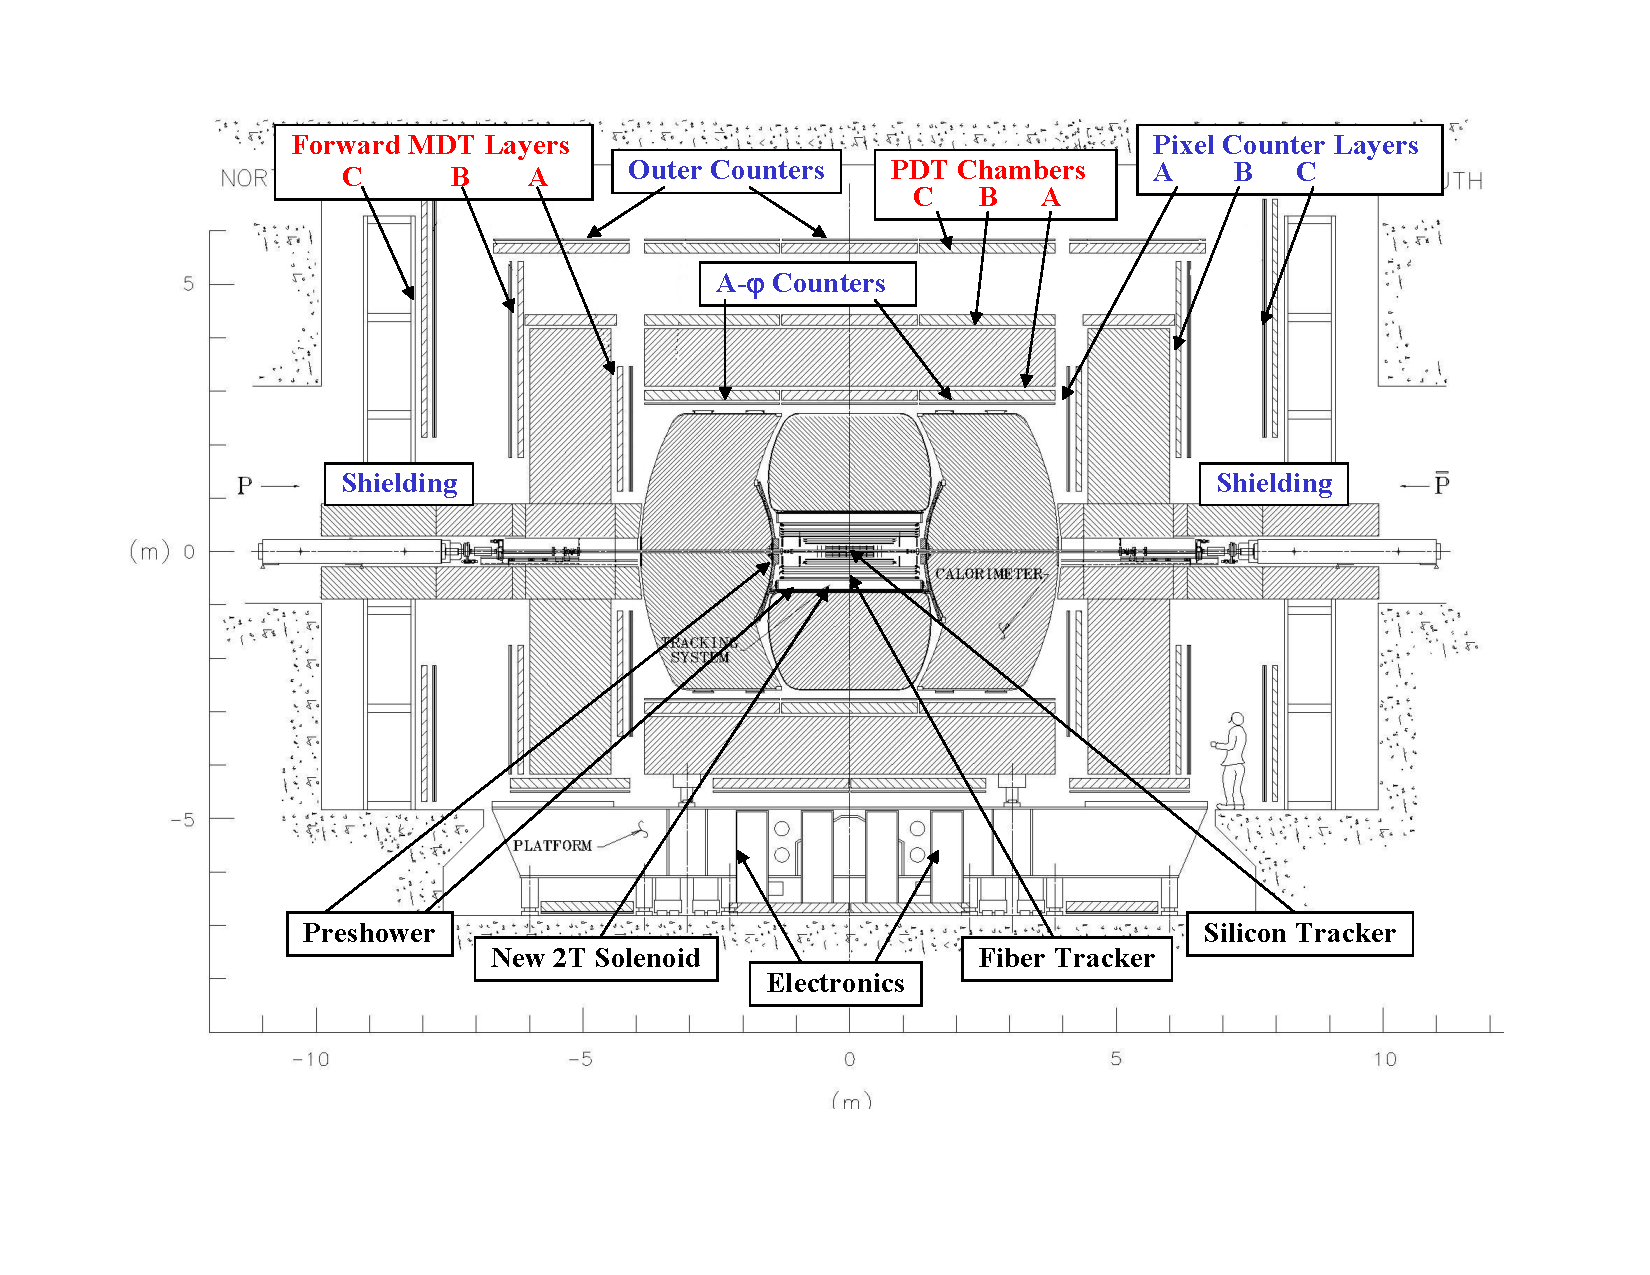
\includegraphics[width=0.9\textwidth]{./Images/41_MD_layout_01}
    \end{figure}
  \end{overlayarea}
\end{frame}

\subsection{Toroidal magnets}
%%%%%% SLIDE
\begin{frame}{\textcolor{Goldenrod}{Muon Tracking System }}
  \begin{overlayarea}{\textwidth}{\textheight}
    % \begin{figure}[h]
    %   \centering
    %   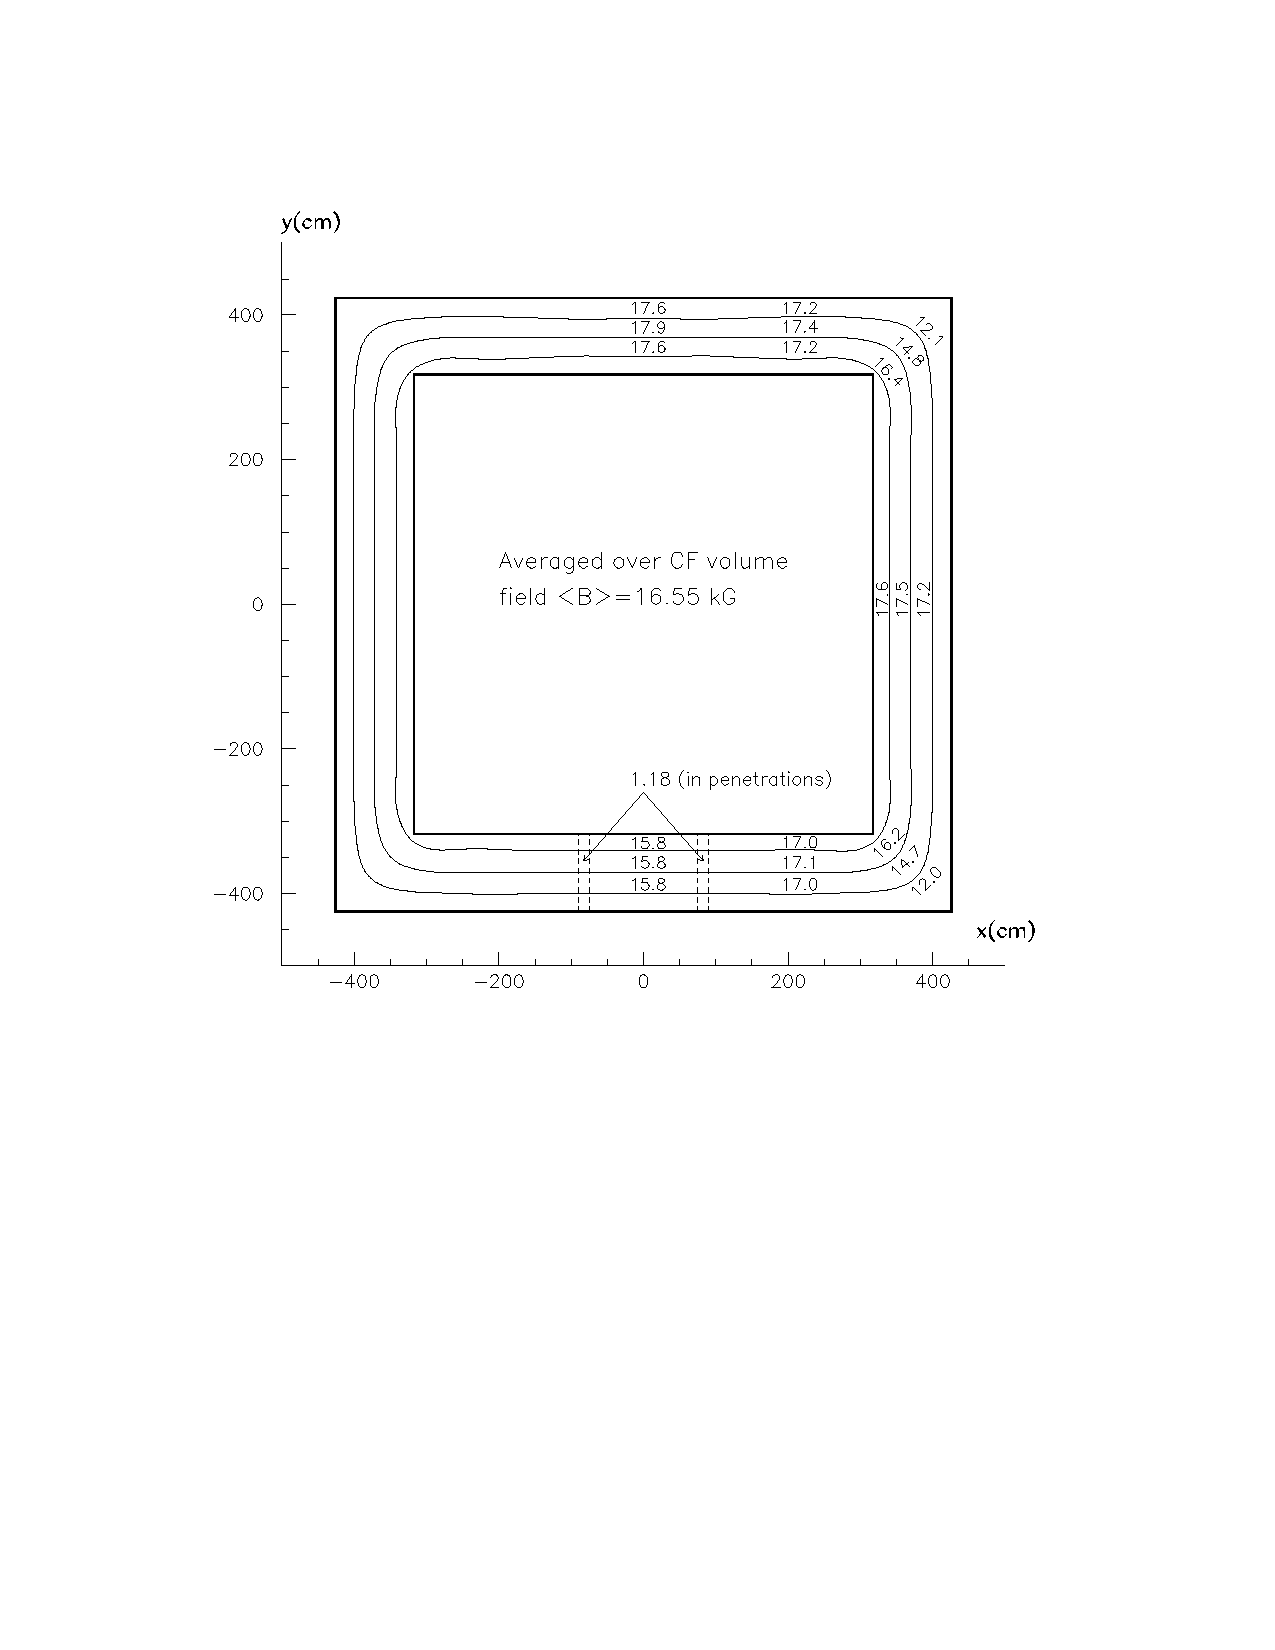
\includegraphics[height=0.4\textheight]{./Images/42_MD_central_magnet}
    %   \caption*{{\scriptsize Magnetic field in the central toroid
    %       magnet. The magnetic field is in $kG$.}}
      
    % \end{figure}
    \itt
  \item \hlt{black}{Why a muon tracking system}\\
    $i)$ enables a low-pT cutoff in the Level 1 muon trigger\\
    $ii)$ allows for cleaner matching with central detector tracks\\
    $iii)$ rejects $\pi/K$ decays\\
    $iv)$ improves the momentum resolution for high
    momentum muons.
  \item \hlt{black}{Toroidal magnet:}\\
    $-$ $8/10$ superconducting coils ($r = 60 cm, l = 250 cm$) carrying
    $1500 A$
    $-$ current reversing switches $\to $ same amount of collected
    data in each plorization
    \tti
  \end{overlayarea}
\end{frame}


\subsection{Central muon detector}
%%%%%% SLIDE
\begin{frame}{\textcolor{Goldenrod}{Muon Tracking System}}
  \begin{overlayarea}{\textwidth}{\textheight}
    \begin{figure}[h]
      \centering
      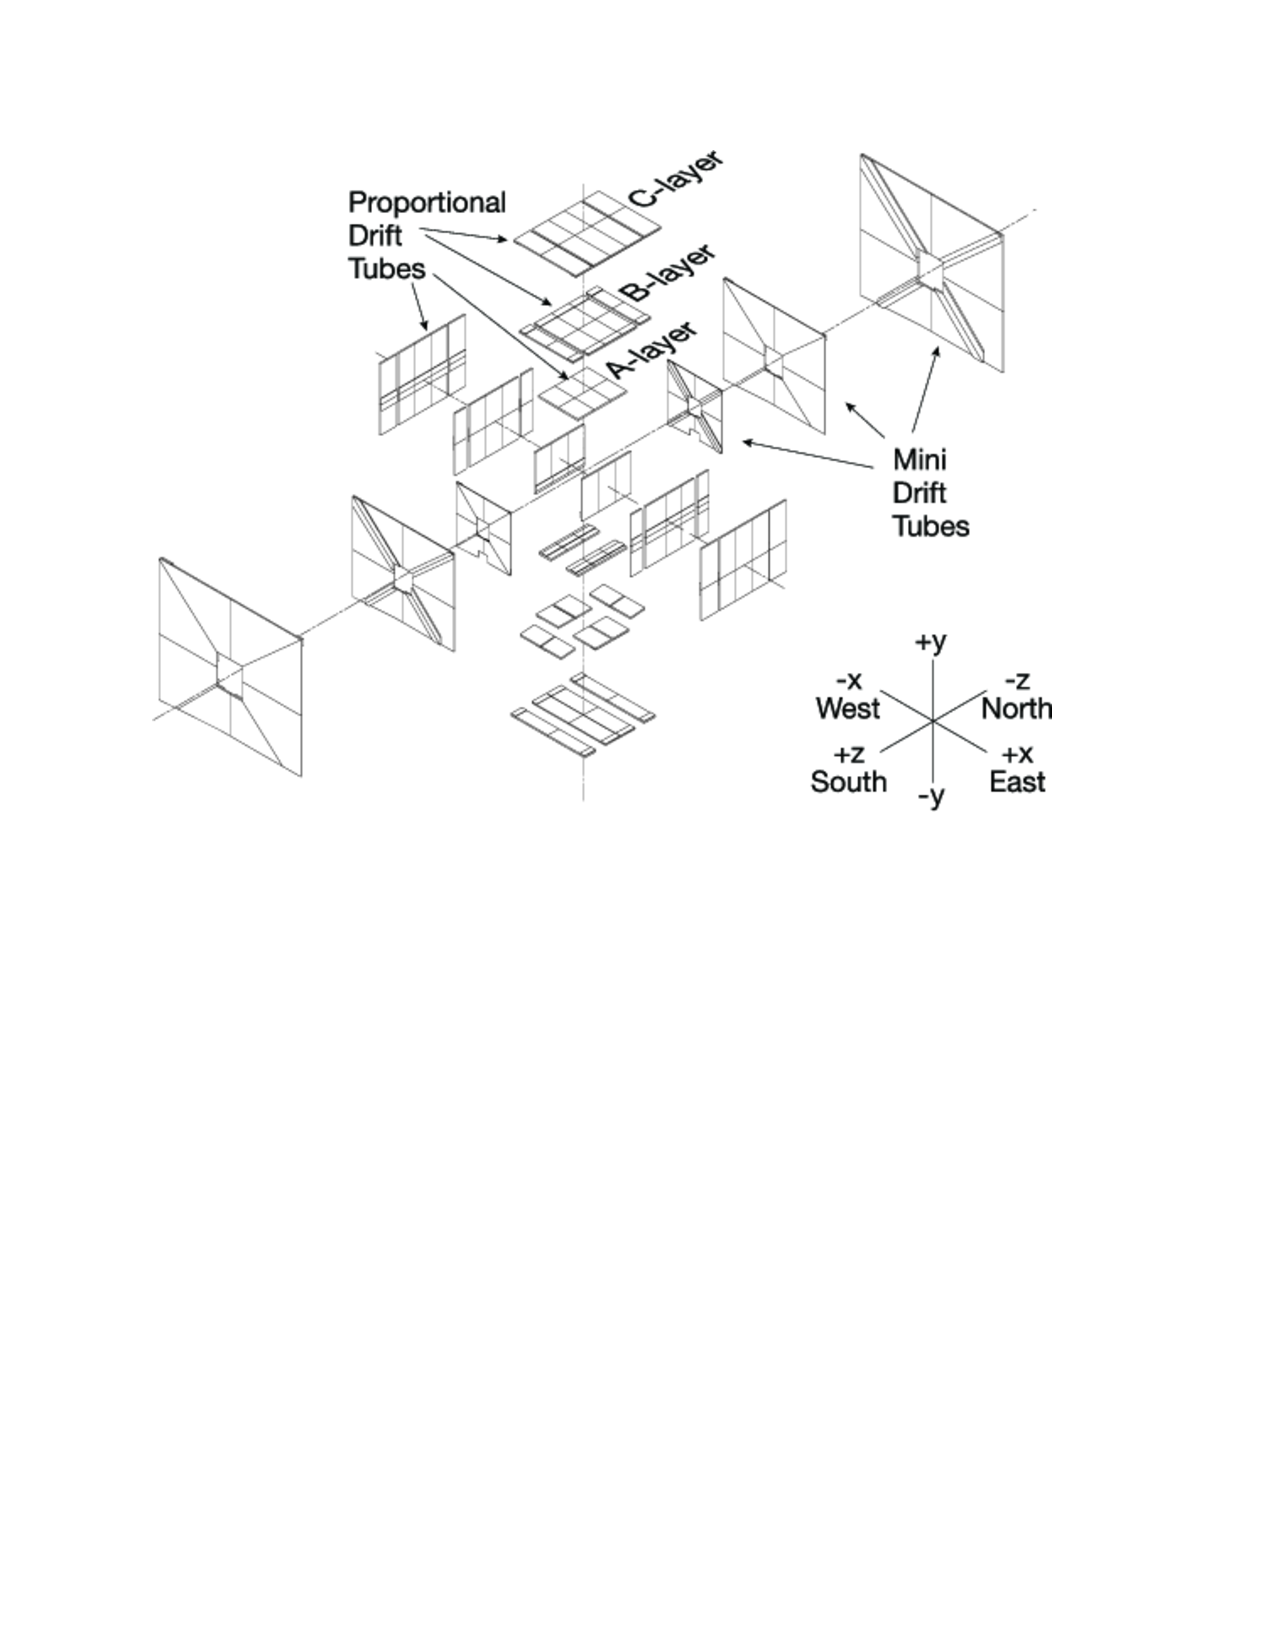
\includegraphics[height=0.4\textheight]{./Images/43_MD_PDT.pdf}
    \end{figure}
    {\small
    \itt
  \item[$\bullet$] 
    three layers of drift chambers, located inside (A layer)
    and outside (B and C layers) of the central toroid\\
    in total $94$ PDT chambers with $6624$ cells.
    
  \item[$\bullet$]
    The $2.8 \times 5.6 m^2$ chambers (3 or 4 decks of PDT), are
    filled with 84\% Argon, 8\% $CF_4$,and 8\% $CH_4$ (fast and
    non-flammable).
    \tti
  }
  \end{overlayarea}
\end{frame}

%%%%%% SLIDE
\begin{frame}{\textcolor{Goldenrod}{Muon Tracking System: PDT}}
  \begin{overlayarea}{\textwidth}{\textheight}
    % \begin{figure}[h]
    %   \centering
    %   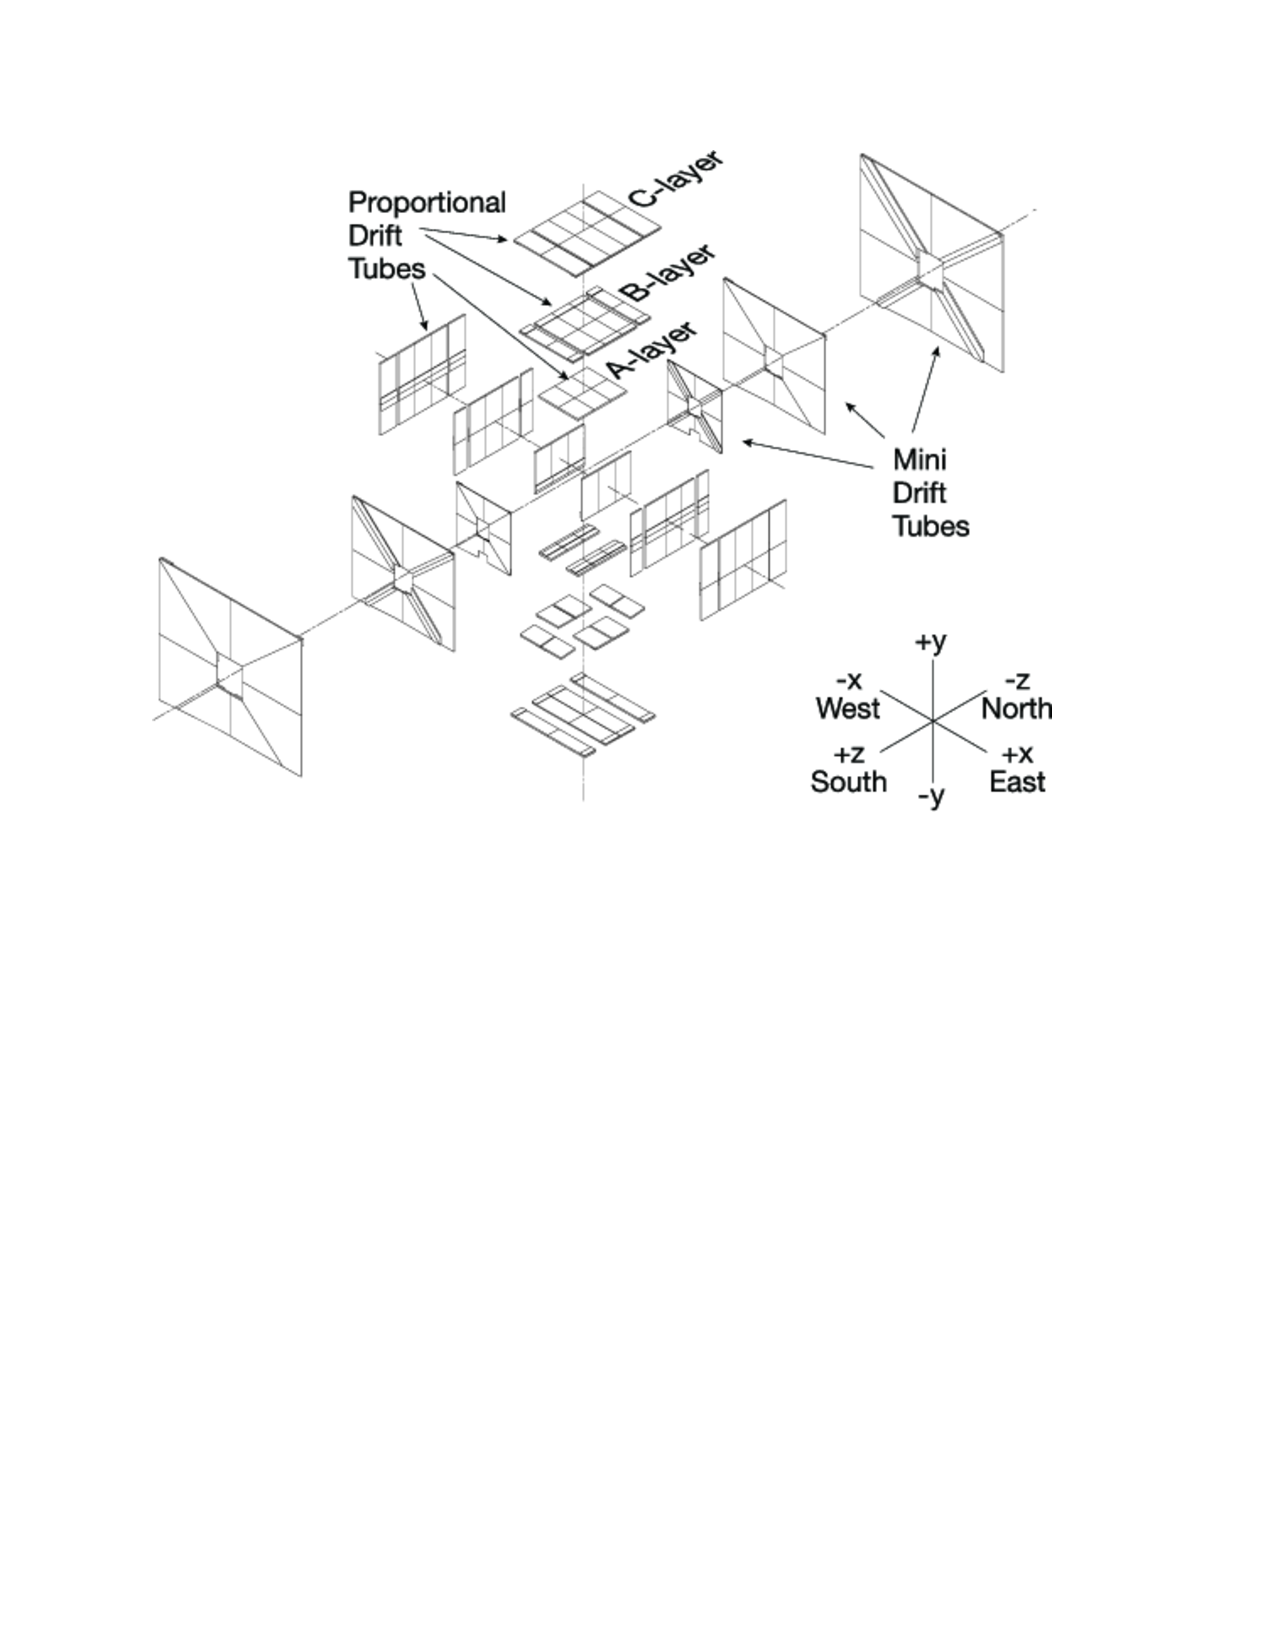
\includegraphics[height=0.4\textheight]{./Images/43_MD_PDT.pdf}
    % \end{figure}
    \itt
  \note{ Each PDT consists of a rectangular shaped
    aluminium enclosure, an anode wire at the center and two cathode
    pads above and below the anode wire.}

  \item[$\circ$] Anodes are held at $4.7 kV$ and electrodes at $2.3 kV$
    The maximum electron drift time in the $10 cm$ wide drift cell is
    $450 ns$
    
  \item[$\circ$] The cathode pads are made of
    thin copper-clad Glasteel
    
  \item[$\circ$] \hlt{black}{For each PDT hit:\\}
    \itt
  \item the electron drift time,
  \item \alert{ $\Delta t$, the difference in the arrival time of the signal
      pulse at the end of the hit cell’s wire and at the end of its readout
      partner’s wire}
  \item the charge deposition on the cathode is measured.
    \tti
  \item[$\circ$]
    \alert{only the A-layer pads are fully instrumented with electronics.
    about 10\% of the B-and C-layer pads are instrumented.}
  \tti
  \end{overlayarea}
\end{frame}

%%%%%% SLIDE
\begin{frame}{\textcolor{Goldenrod}{Muon Forward Tracking System}}
  \begin{overlayarea}{\textwidth}{\textheight}
    \begin{figure}[h]
      \centering
      %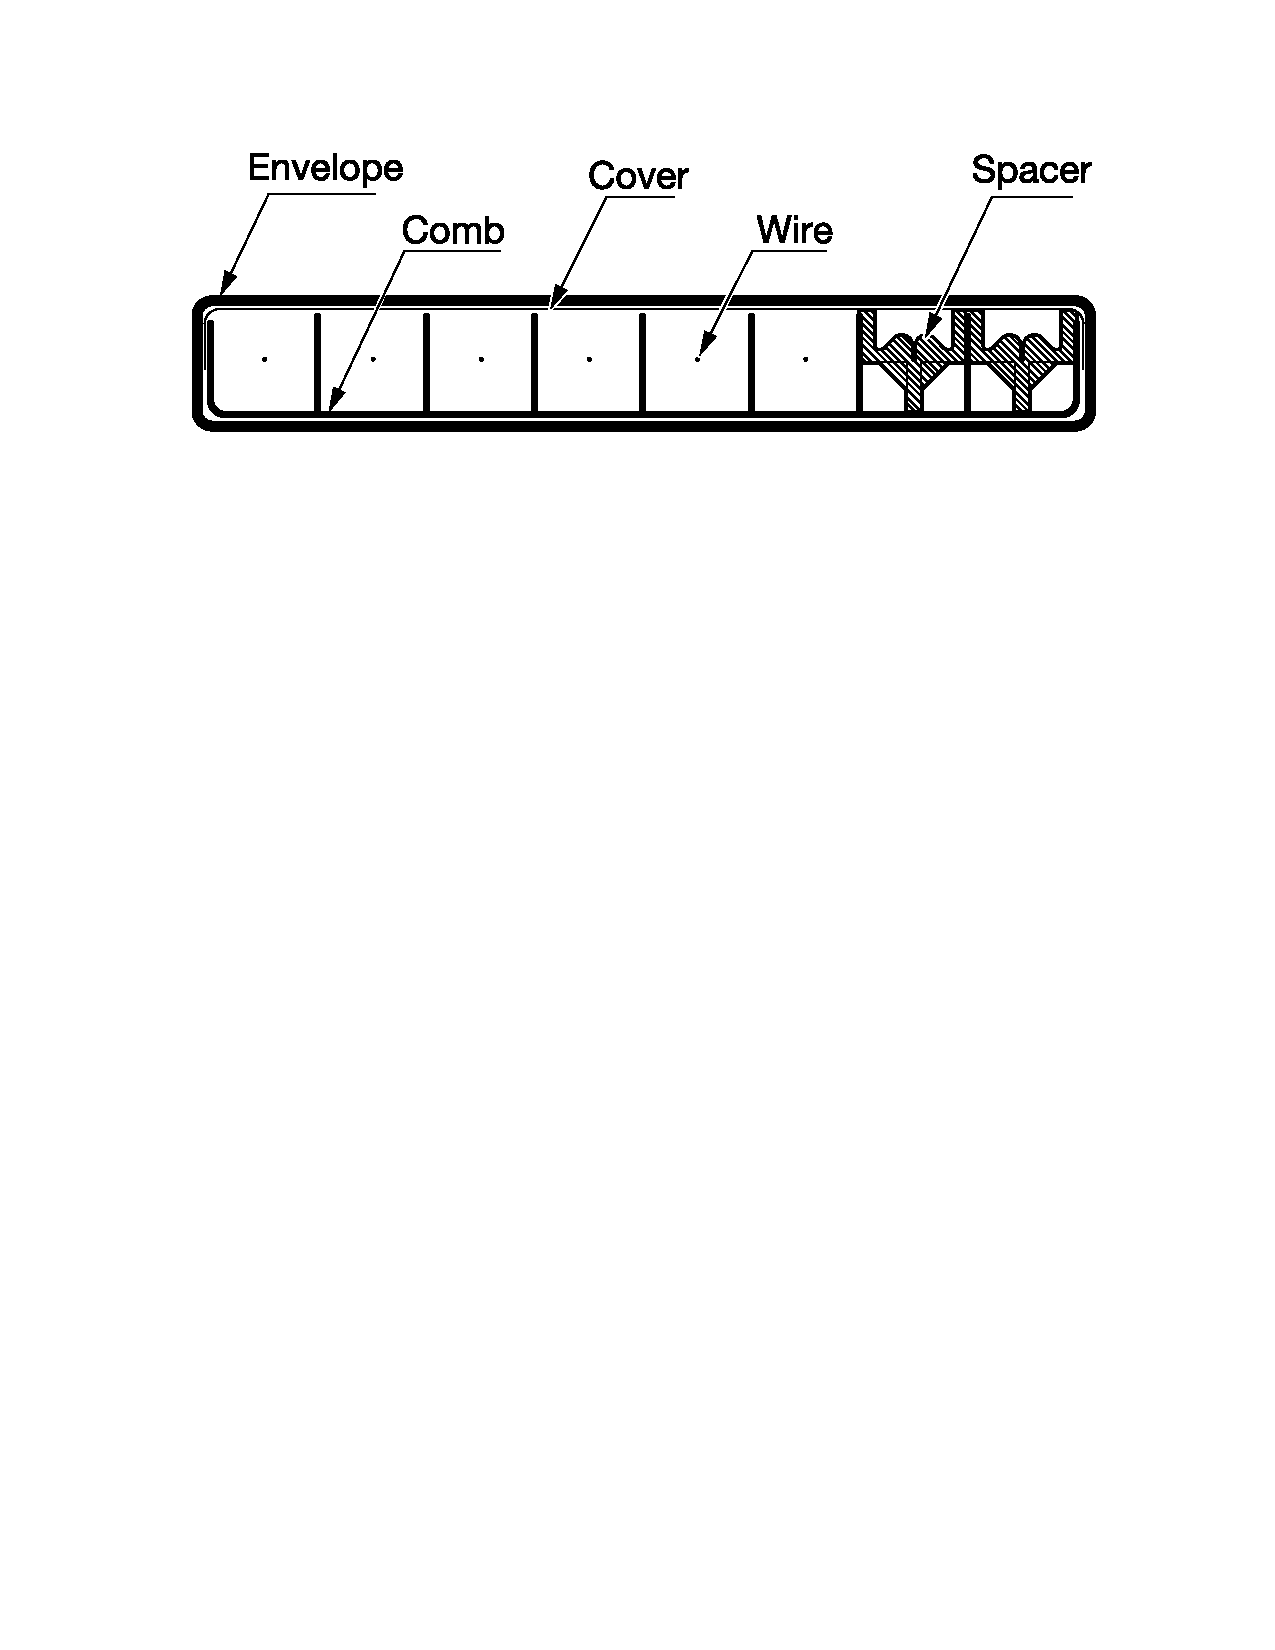
\includegraphics[height=0.4\textheight, width=0.5\textwidth]{./Images/45_MD_miniPDT_01.pdf}
      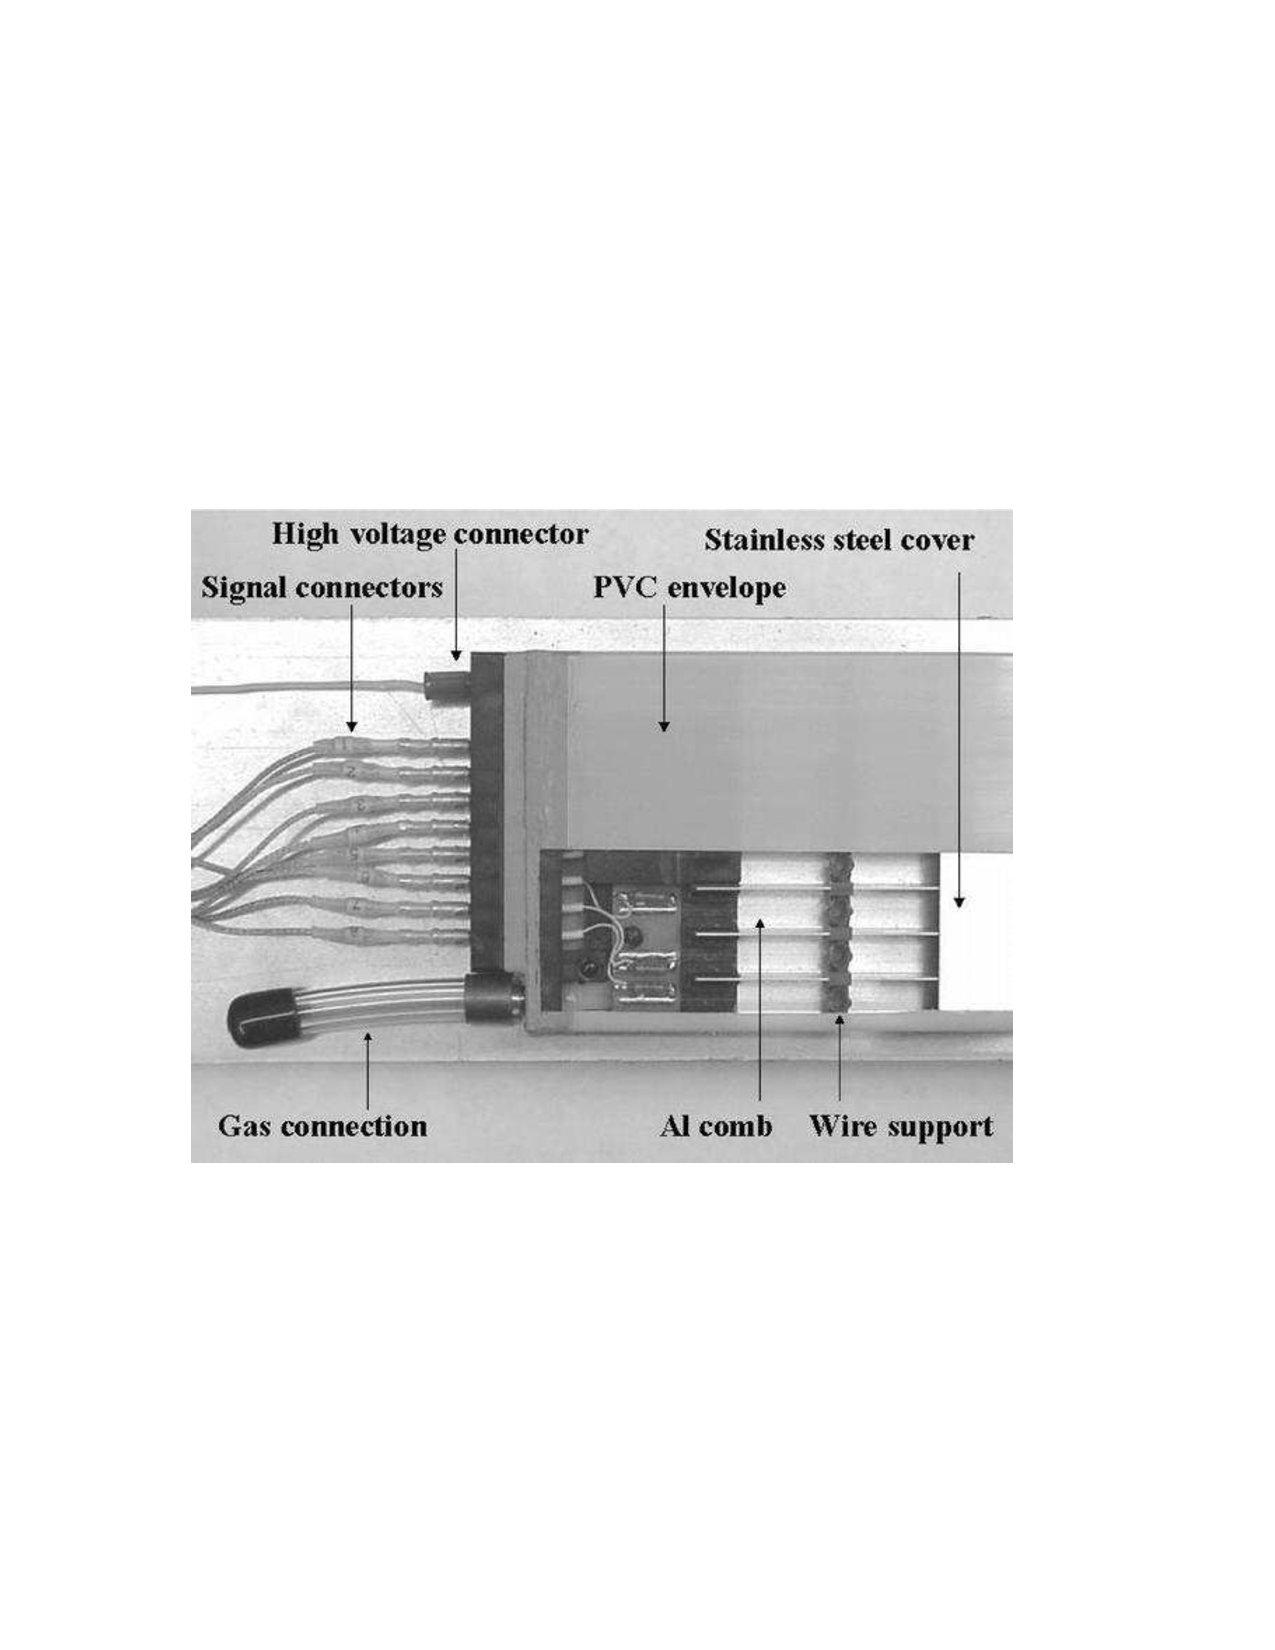
\includegraphics[height=0.4\textheight]{./Images/45_MD_miniPDT_02.pdf}
    \end{figure}
    \itt
  \item The MDT system consists of 6080 mini drift tubes ($9.4 \times
    9.4 mm^2$) that are assembled into six layers of eight octants each.
  \item \hlt{blue}{anodes:} eight $50 \mu m$ gold-plated tungsten
  \item \hlt{Blue}{gas mixture:} 90\% $CF_4$ and 10\% $CH_4$.
    \tti
  \end{overlayarea}
\end{frame}

%%%%%% SLIDE
\begin{frame}{\textcolor{Goldenrod}{Muon Forward Tracking System}}
  \begin{overlayarea}{\textwidth}{\textheight}
    \begin{figure}[h]
      \centering
      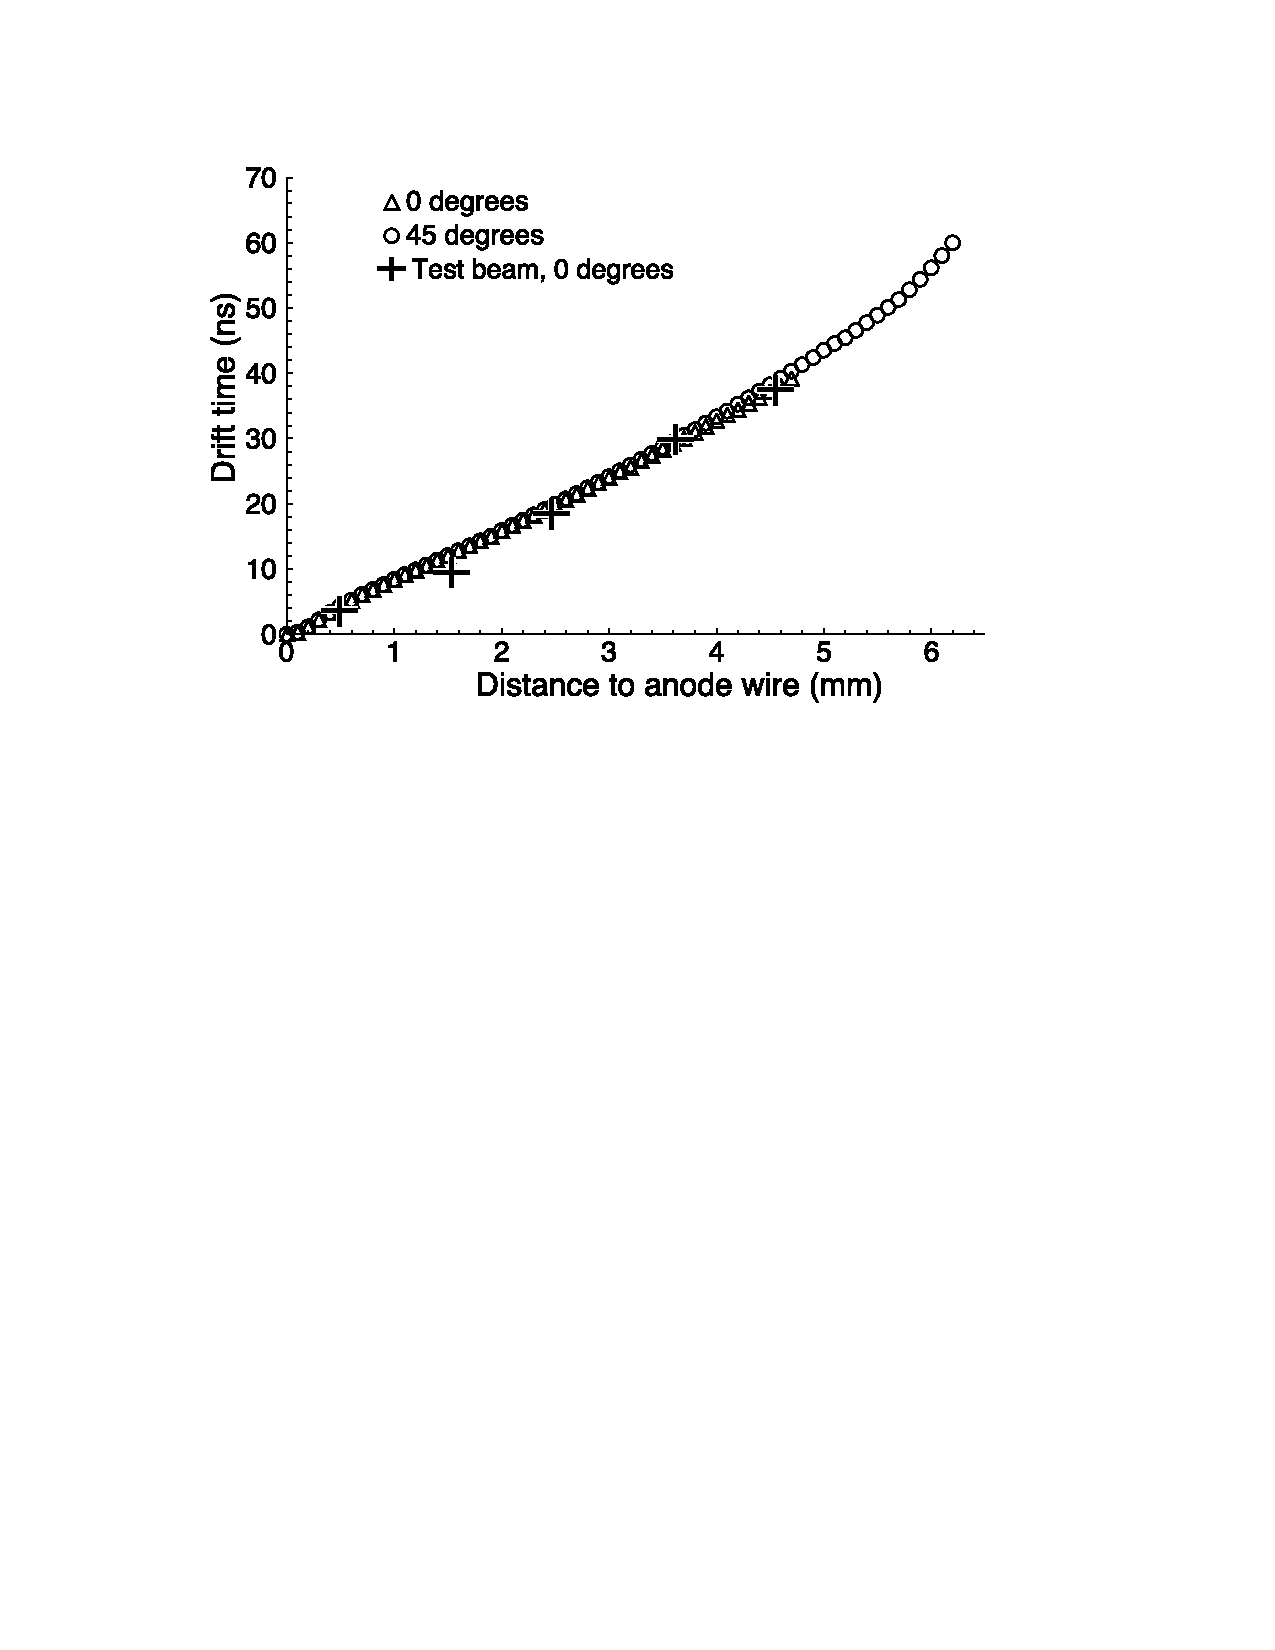
\includegraphics[height=0.35\textheight]{./Images/45_MD_miniPDT_03.pdf}
    \end{figure}
    \itt
  \item[$\circ$]
    each anode wire is
    connected to an amplifier discriminator board (ADB)\\
    
    output logical differential signals from the ADB are sent to
    digitizing electronics which measure the signal arrival time with
    an accuracy of 18.8 ns.
    
    \note{This large time bin (equal to the Tevatron RF bucket size since
      the main accelerator clock is 53 MHz) limits the coordinate
      resolution of the MDTs and was selected to reduce the cost of
      almost 50,000 TDCs (time-to-digital converters). Hit information
      is sent to the trigger and data acquisition systems; the data
      acquisition system also receives drift times.}
  \item[$\circ$]
    tracking efficiency $\approx 99$\% perpendicular to the MDT plane\\
    overall $\approx 95$\% (due to the wall thickness and PVC sleeves) 
    \tti
  \end{overlayarea}
\end{frame}


%%%%%% SLIDE
\begin{frame}{\textcolor{Goldenrod}{Muon Scintillation Counters}}
  \begin{overlayarea}{\textwidth}{\textheight}
    \begin{figure}[h]
      \centering
      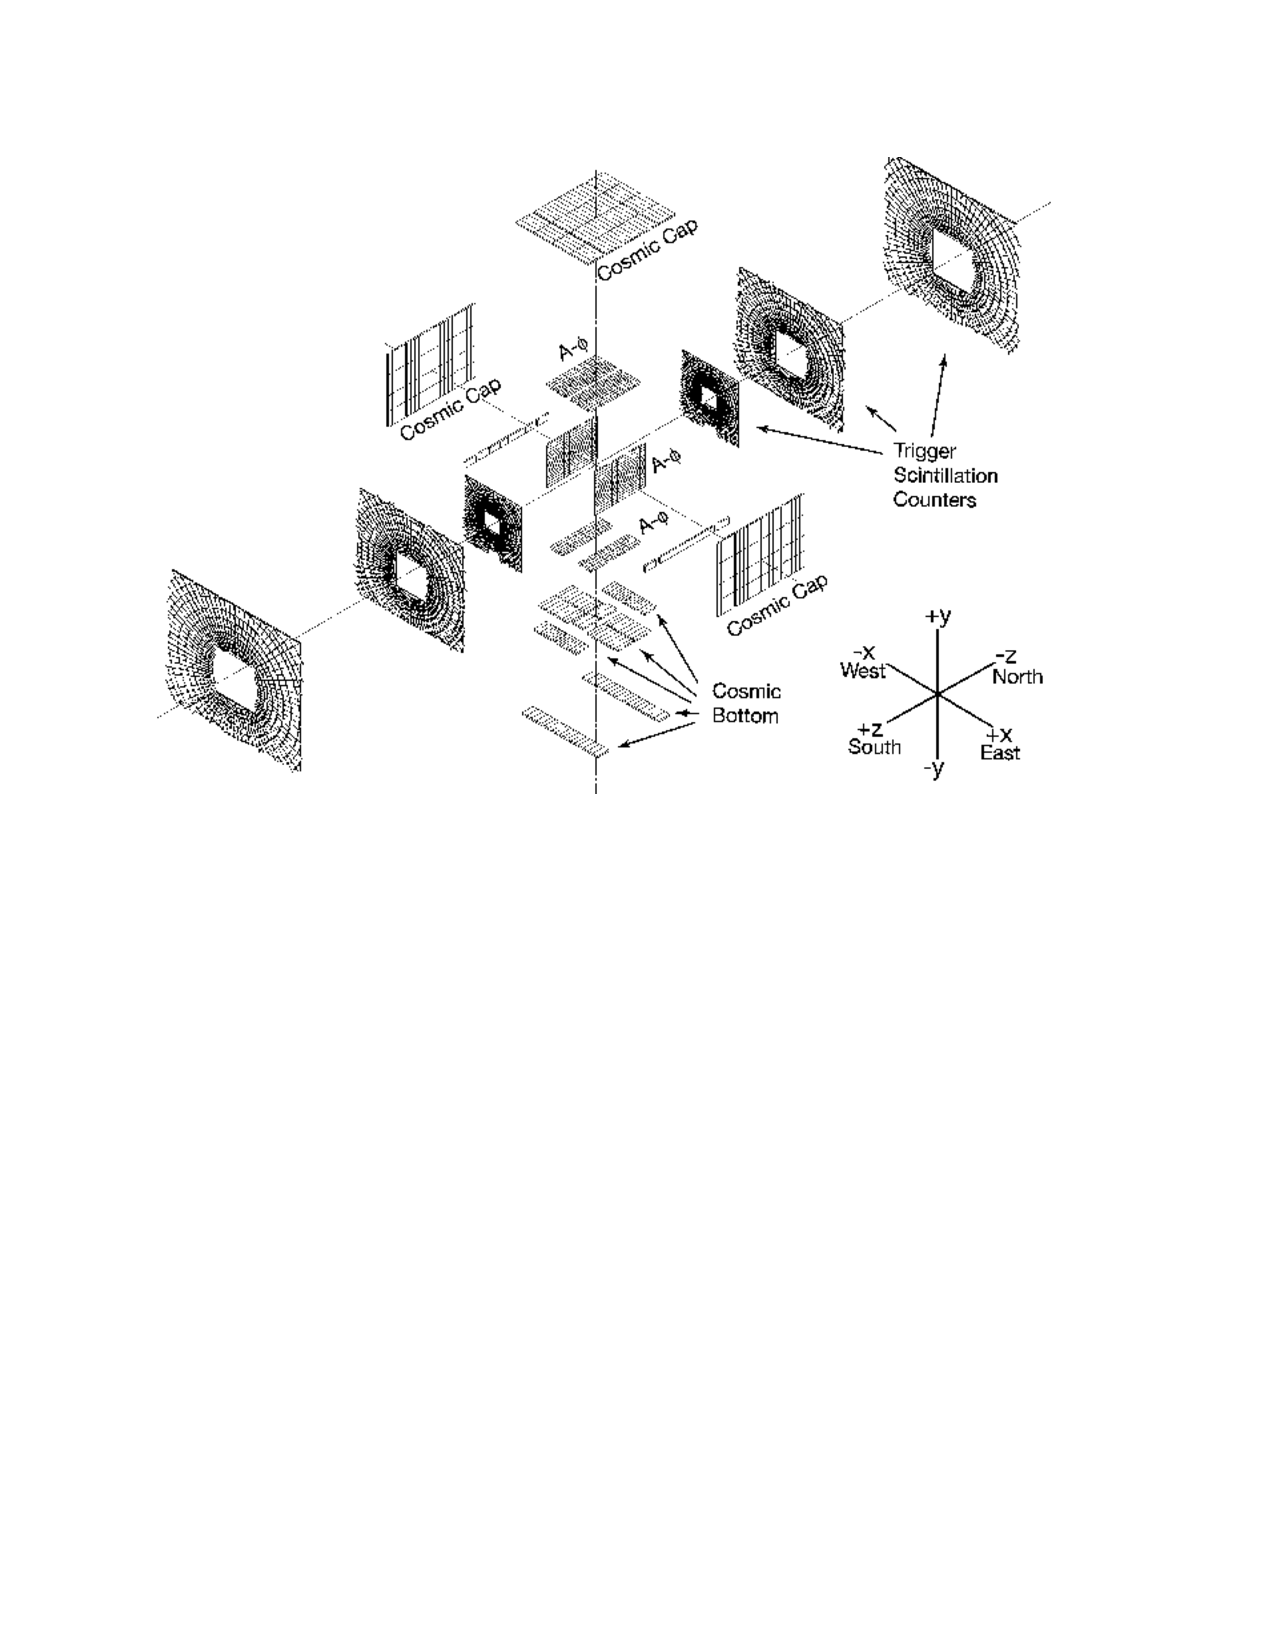
\includegraphics[height=0.4\textheight]{./Images/44_MD_Sintillators}
    \end{figure}
    
    \itt

  \item
    2/3 central/forward scintillation counters layers.
    
  \item provide a fast timing signal to associate a muon in a PDT with the
    appropriate bunch crossing and discriminate against the cosmic ray
    background.
    \tti
  \end{overlayarea}
\end{frame}

\subsection{Forward muon system}

%%%%%% SLIDE
\begin{frame}{\textcolor{Goldenrod}{Muon $A\phi$ Scintillation Counters}}
  \begin{overlayarea}{\textwidth}{\textheight}
    \begin{figure}[h]
      \centering
      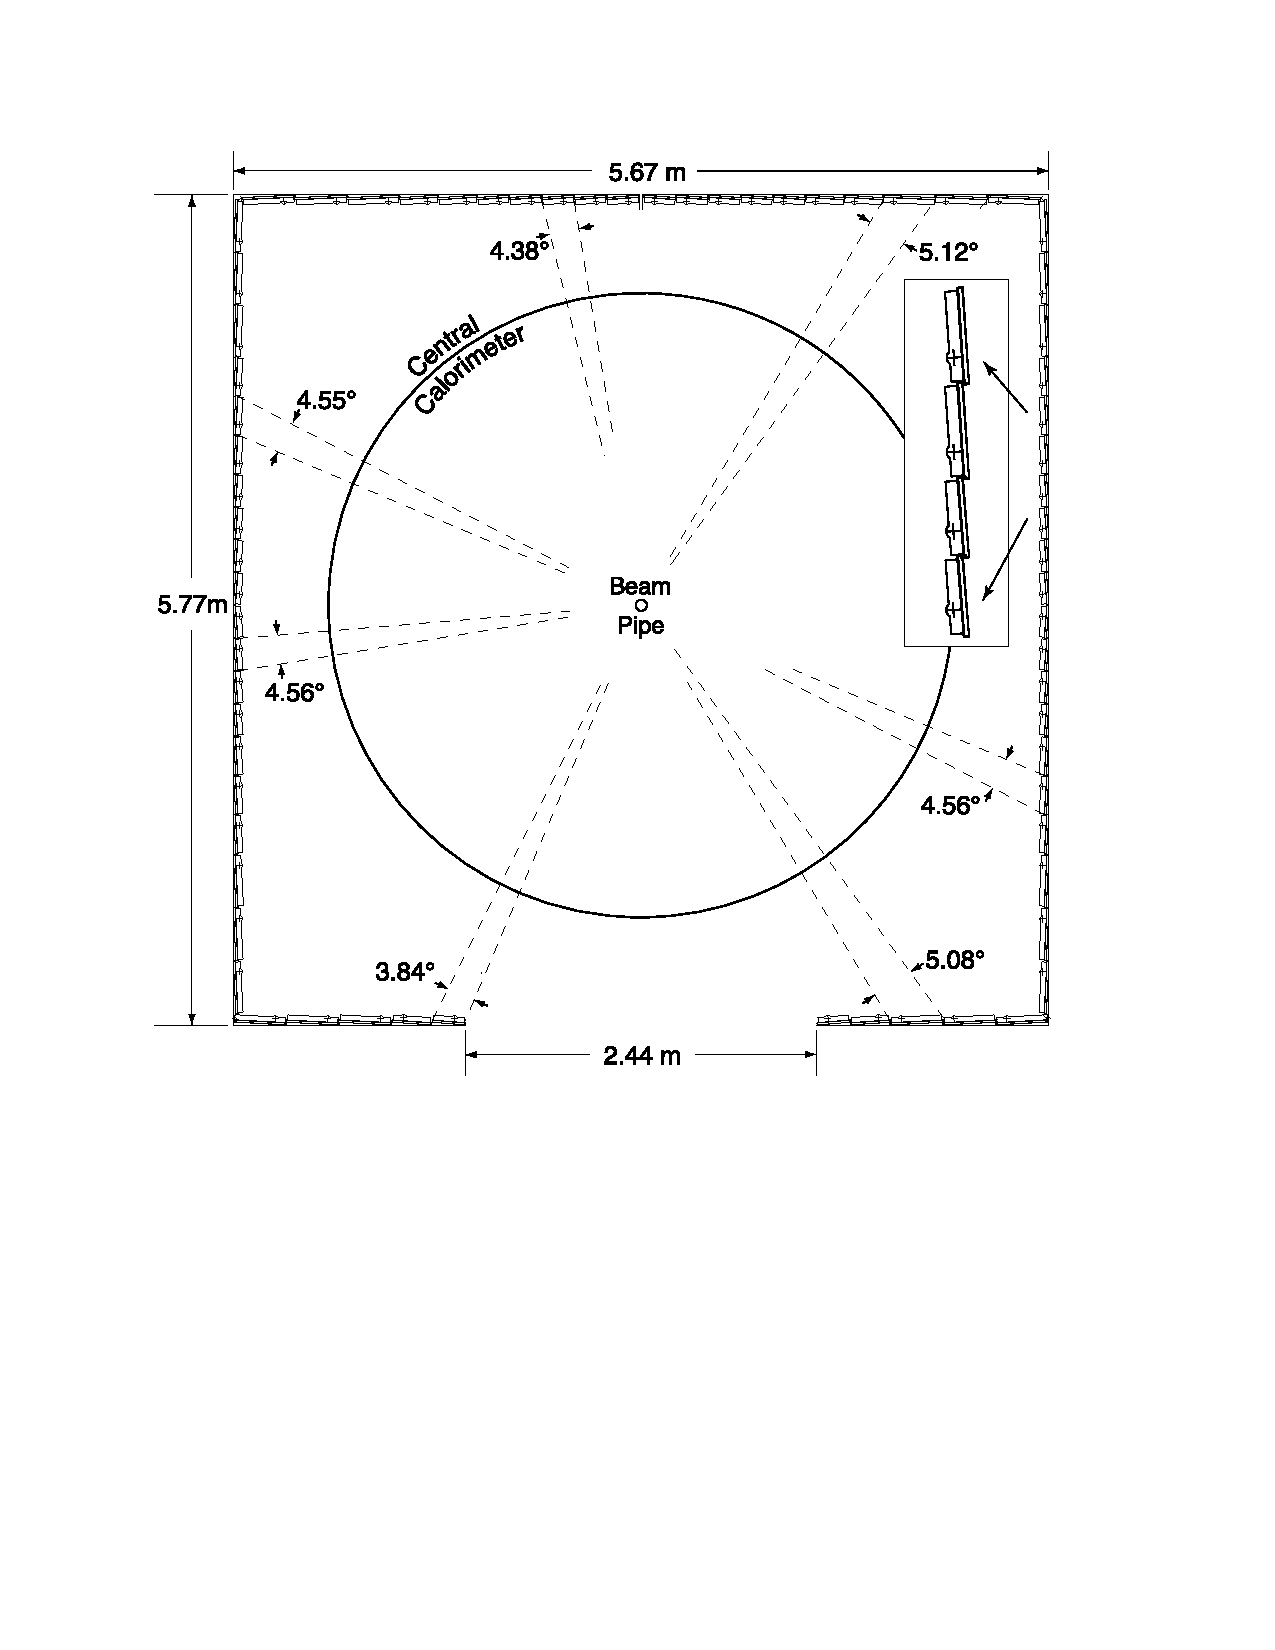
\includegraphics[height=0.4\textheight, width=0.4\textwidth]{./Images/46_MD_Scint_01.pdf}
      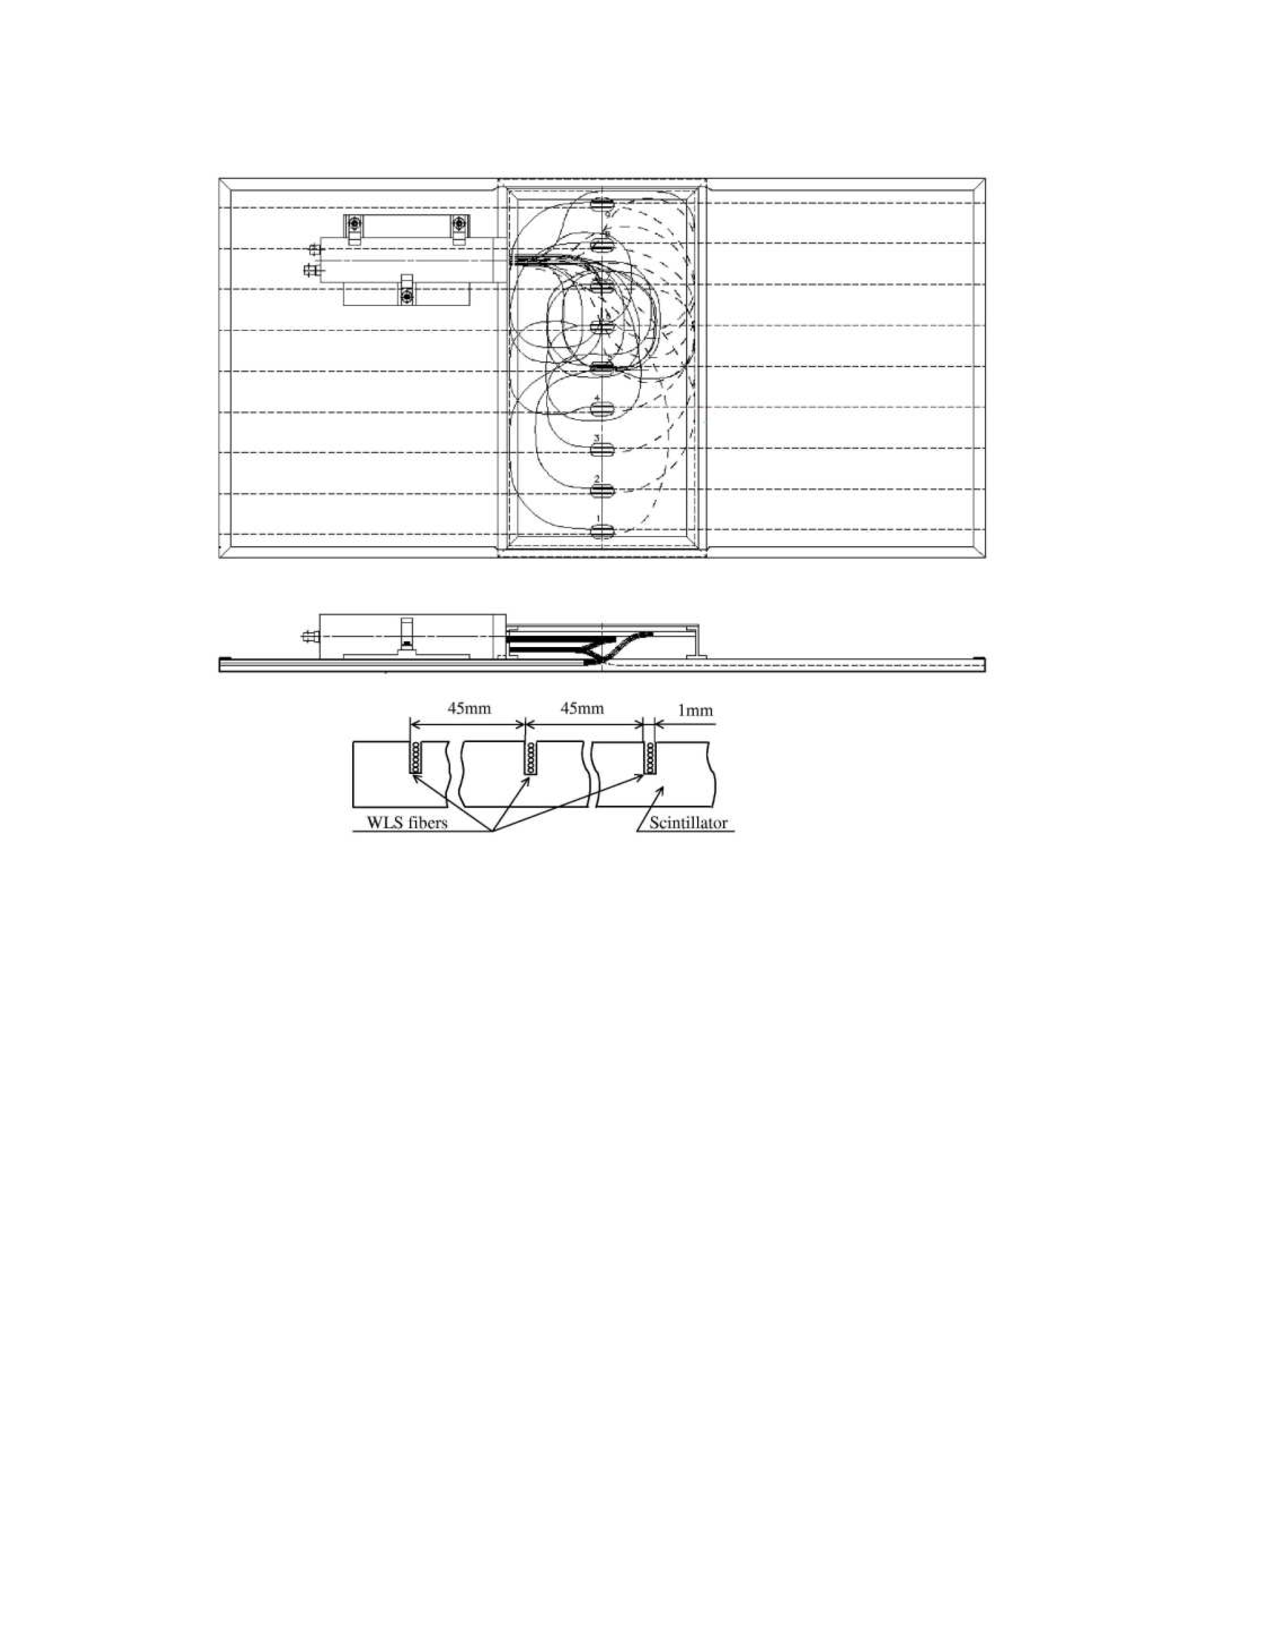
\includegraphics[height=0.4\textheight, width=0.5\textwidth]{./Images/46_MD_Scint_02.pdf}
    \end{figure}
    \itt

  \item
    Nine barrels of counters cover $|\eta| < 1.0$.

  % \item each counter is $84.5 cm$ cm long. Twenty
  %   counter columns, of three different widths, cover one quadrant in
  %   the azimuthal direction.
    
  \item
    \alert{$\delta \phi \approx 4.5^{\circ}; \delta l \approx 80 cm$
      to match CFT segmentation and time resolution of PDT}
    % central fiber tracker trigger (Section 9.1.3) segmentation. The
    % longitudinal segmentation is $33.25”$ which provides the necessary
    % time resolution and a match to the size of the PDTs
  \item
    $12.7-mm-thick$ BICRON $404A$ scintillator with BICRON BCF $92$
    wavelength shifter fiber
    
  % \item
  %   The grooves are machined $4.5 cm$ apart and $6 mm$ deep and run from
  %   the center of the counter to its edge. Six individual fibers are
  %   glued into each groove and tapered out of the groove at the middle
  %   of the counter.
    
  % \item
  %   Fibers from 10 to 16 grooves are combined into a single bundle
  %   that directs light to a 25-mm-diameter green-extended 115M
  %   phototube
    
  %   They are made from grooved $0.5''$ Bicron 404A scintillator with
  %   Bicron BCF 91A and Kuraray Y11 wave-shifting fibers glued into
  %   the grooves using Bicron 600 optical epoxy.
  % \item There are 240
  %   counters, $25"$ wide, and $81.5”-113”$ long. The counters are
  %   positioned with their width along $z$ and length along $\phi$. The
  %   grooves are $1.75 mm$ deep and $4 mm$ wide; they run along the length
  %   of the counter,
    \tti
  \end{overlayarea}
\end{frame}


%%%%%% SLIDE
\begin{frame}{\textcolor{Goldenrod}{Muon $A\phi$ Scintillation Counters Performance }}
  \begin{overlayarea}{\textwidth}{\textheight}
    \begin{figure}[h]\centering
      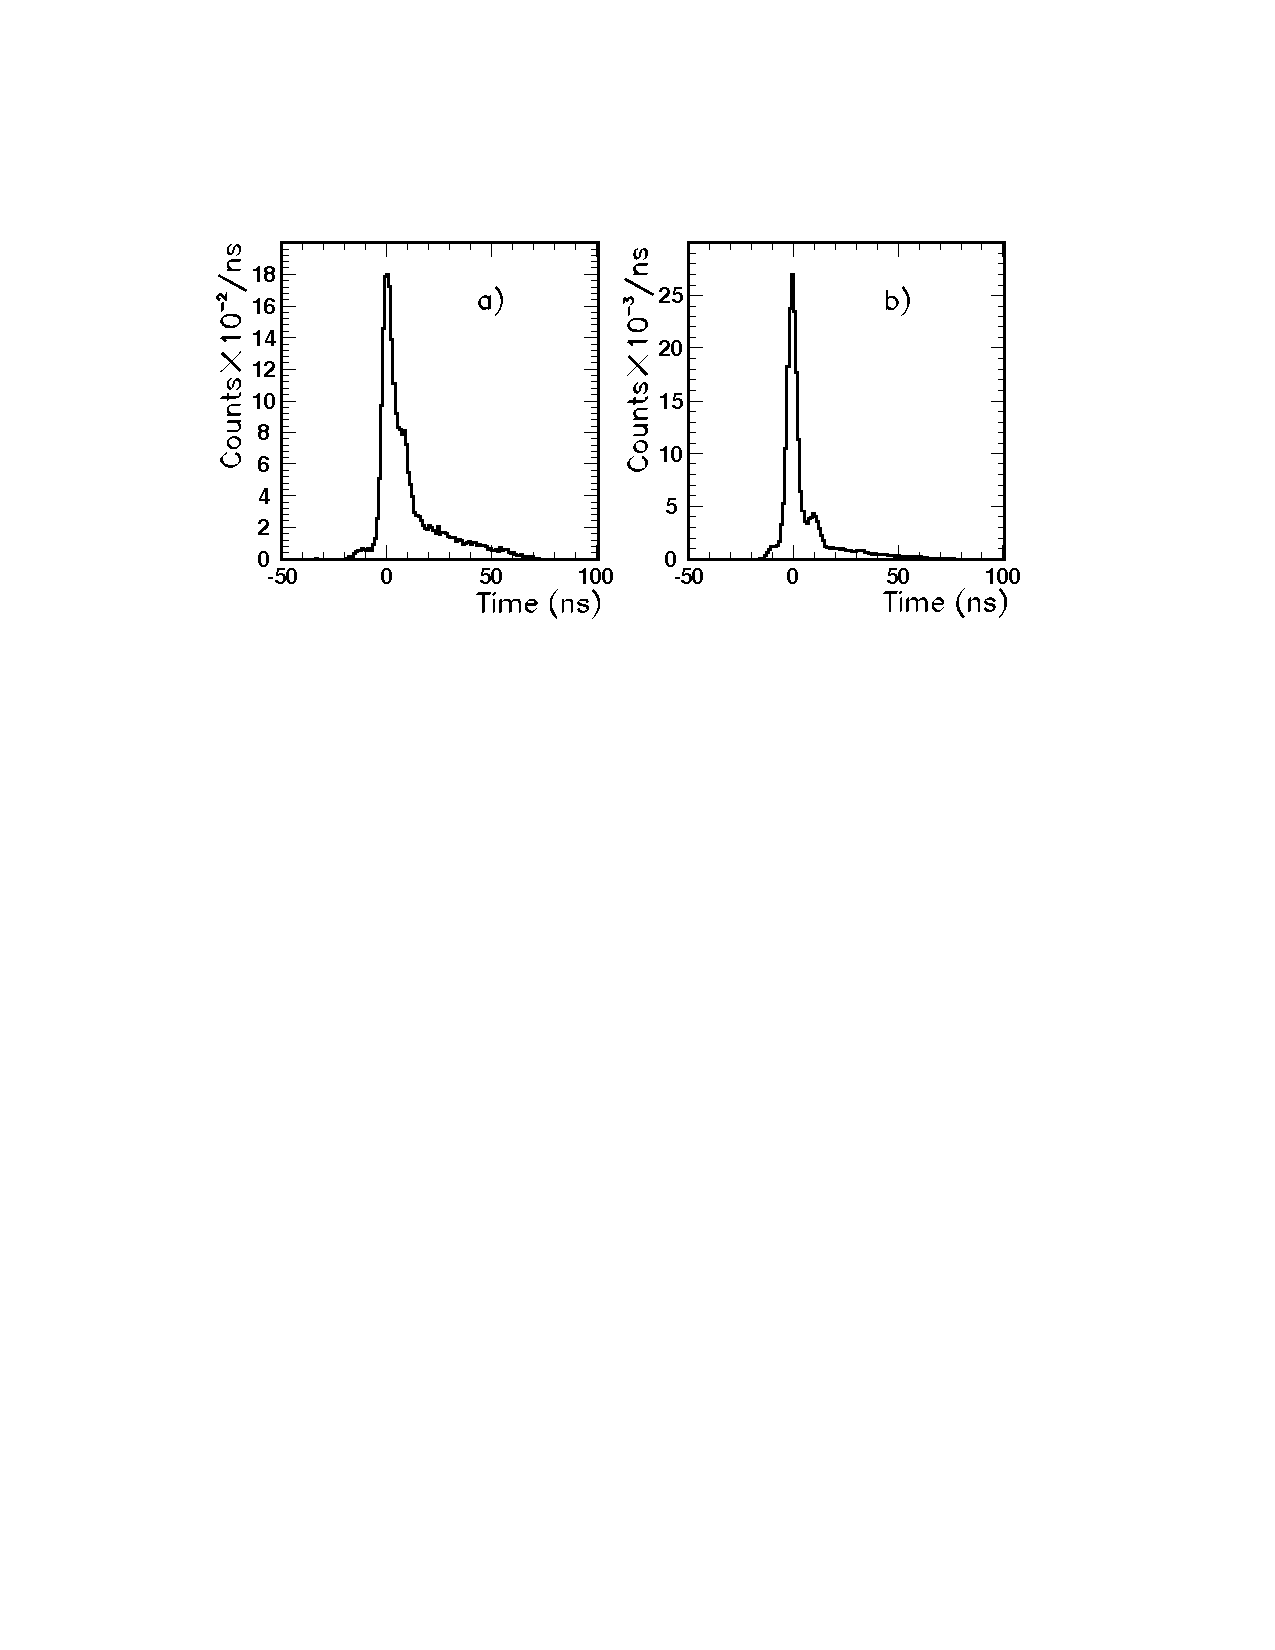
\includegraphics[height=0.35\textheight]{./Images/46_MD_Scint_03}
    \caption*{{\scriptsize The time-of-arrival distributions recorded by $A\phi$ counters in
        events triggered by a) all triggers b) muon triggers only.}}
    \end{figure}
    
    \itt
  \item the peaks around zero in both figures are from muons
    originating at the interaction region
  \item
    \alert{the time resolution of all $630$ $A\phi$ counters combined is
    $\sigma_t = 2.5 ns$}
    
    \note{
      The time-of-arrival distribution shown in Fig. 12a includes a
      significant number of late hits from the various background
      sources
      A secondary peak near 10 ns that is visible  is caused
      by backscattered particles from the edges of calorimeter}
   \tti
  \end{overlayarea}
\end{frame}


%%%%%% SLIDE
\begin{frame}{\textcolor{Goldenrod}{Muon Forward Scintillation Counters}}
  \(
  \<{0.7\textwidth}
  \itt
  \item[$\bullet$] $4214$ trapezoidal counters are arranged in an $r-\phi$ geometry in about twelve
    concentric zones in the radial direction($1.0 < |\eta| < 2.0$)
  \item[$\bullet$] the segmentation:\\
    $i)$ matches the $\phi$ segmentation of the CFT\\
    $ii)$ the minimum muon trigger momentum threshold\\
    $iii)$ muon multiple scattering in the toroids\\
    $iv)$ \alert{background trigger rates due to accidental coincidences
    (combinatoric background rejection scales as $N^m$ for m layers of
    N counters.)}
    \tti
    \>
    \<{0.45\textwidth}
    \img{47_MD_forward_pixels_01.pdf}
    \>
    \)
\end{frame}


%%%%%% SLIDE
\begin{frame}{\textcolor{Goldenrod}{Muon Forward Scintillation Counters}}
  \begin{overlayarea}{\textwidth}{\textheight}
    \begin{figure}[h]\centering
      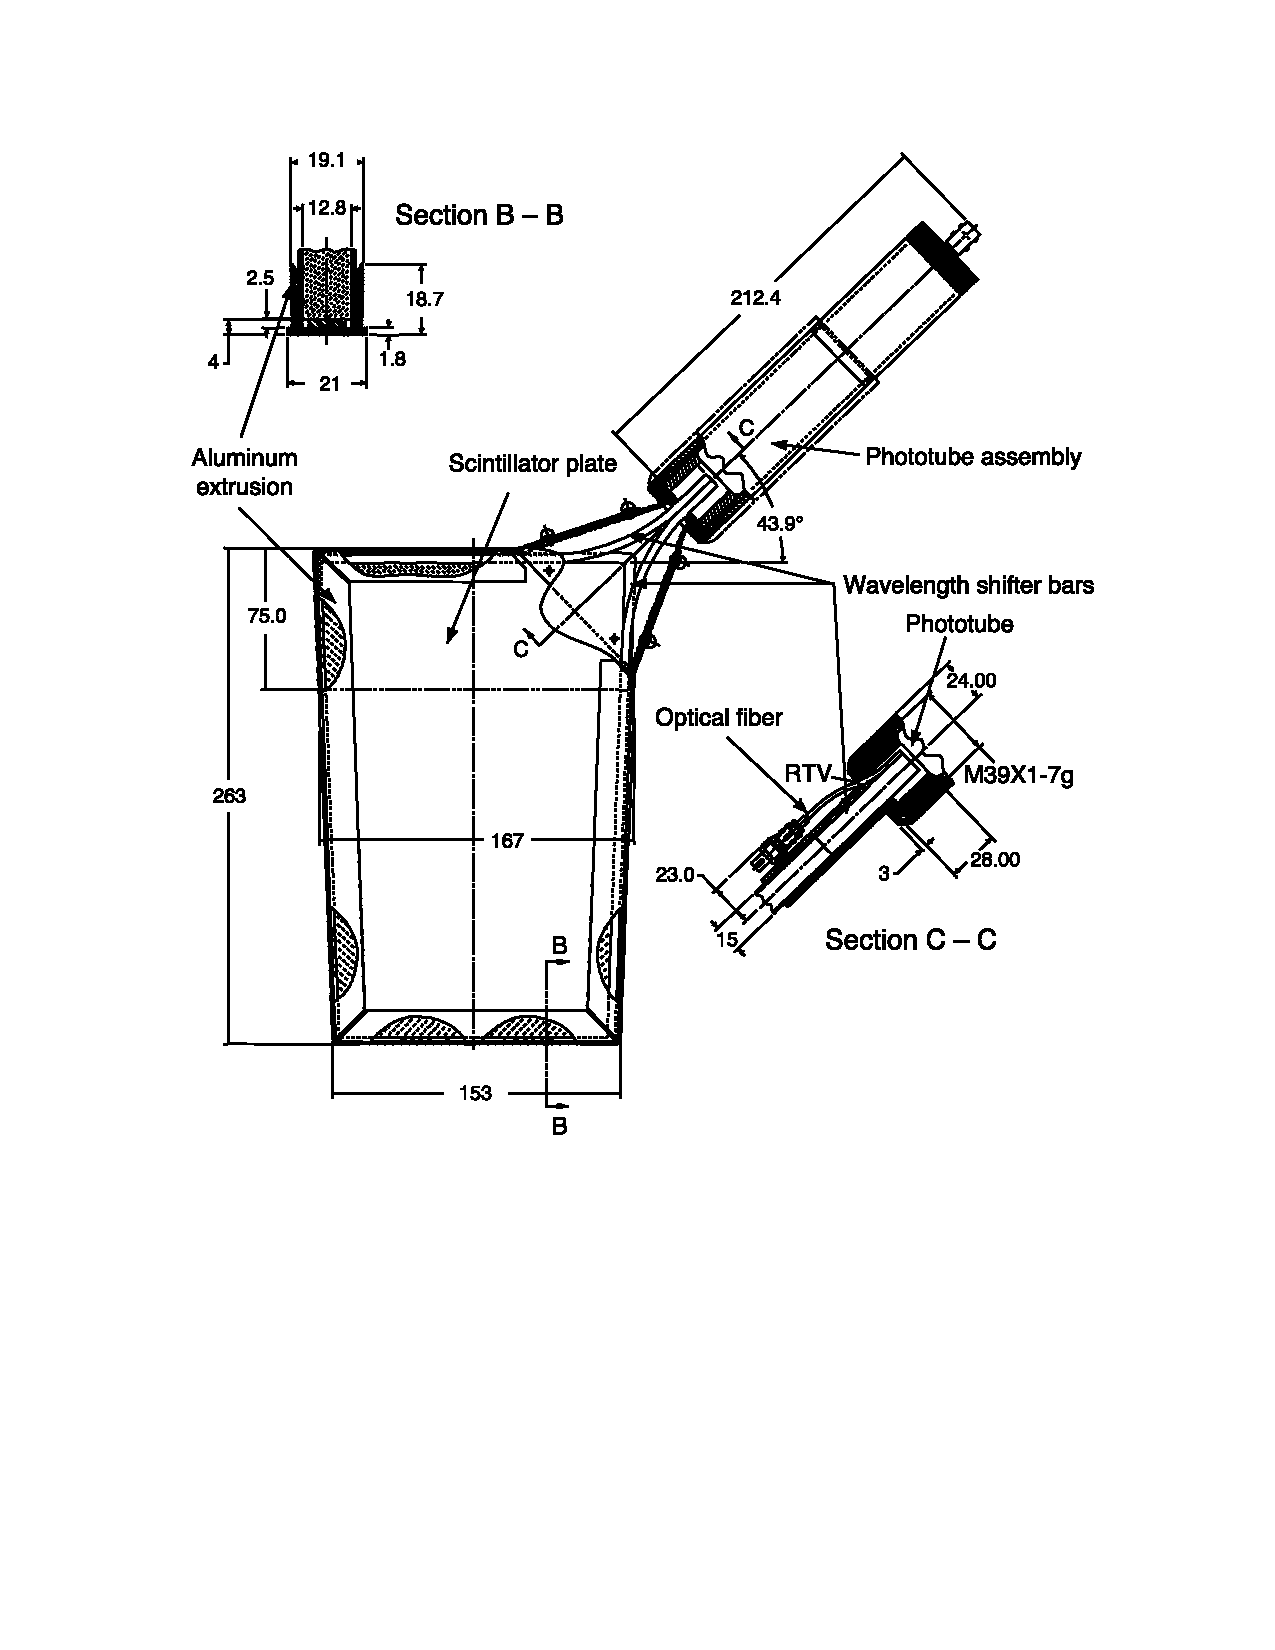
\includegraphics[height=0.65\textheight]{./Images/47_MD_forward_pixels_02.pdf}
      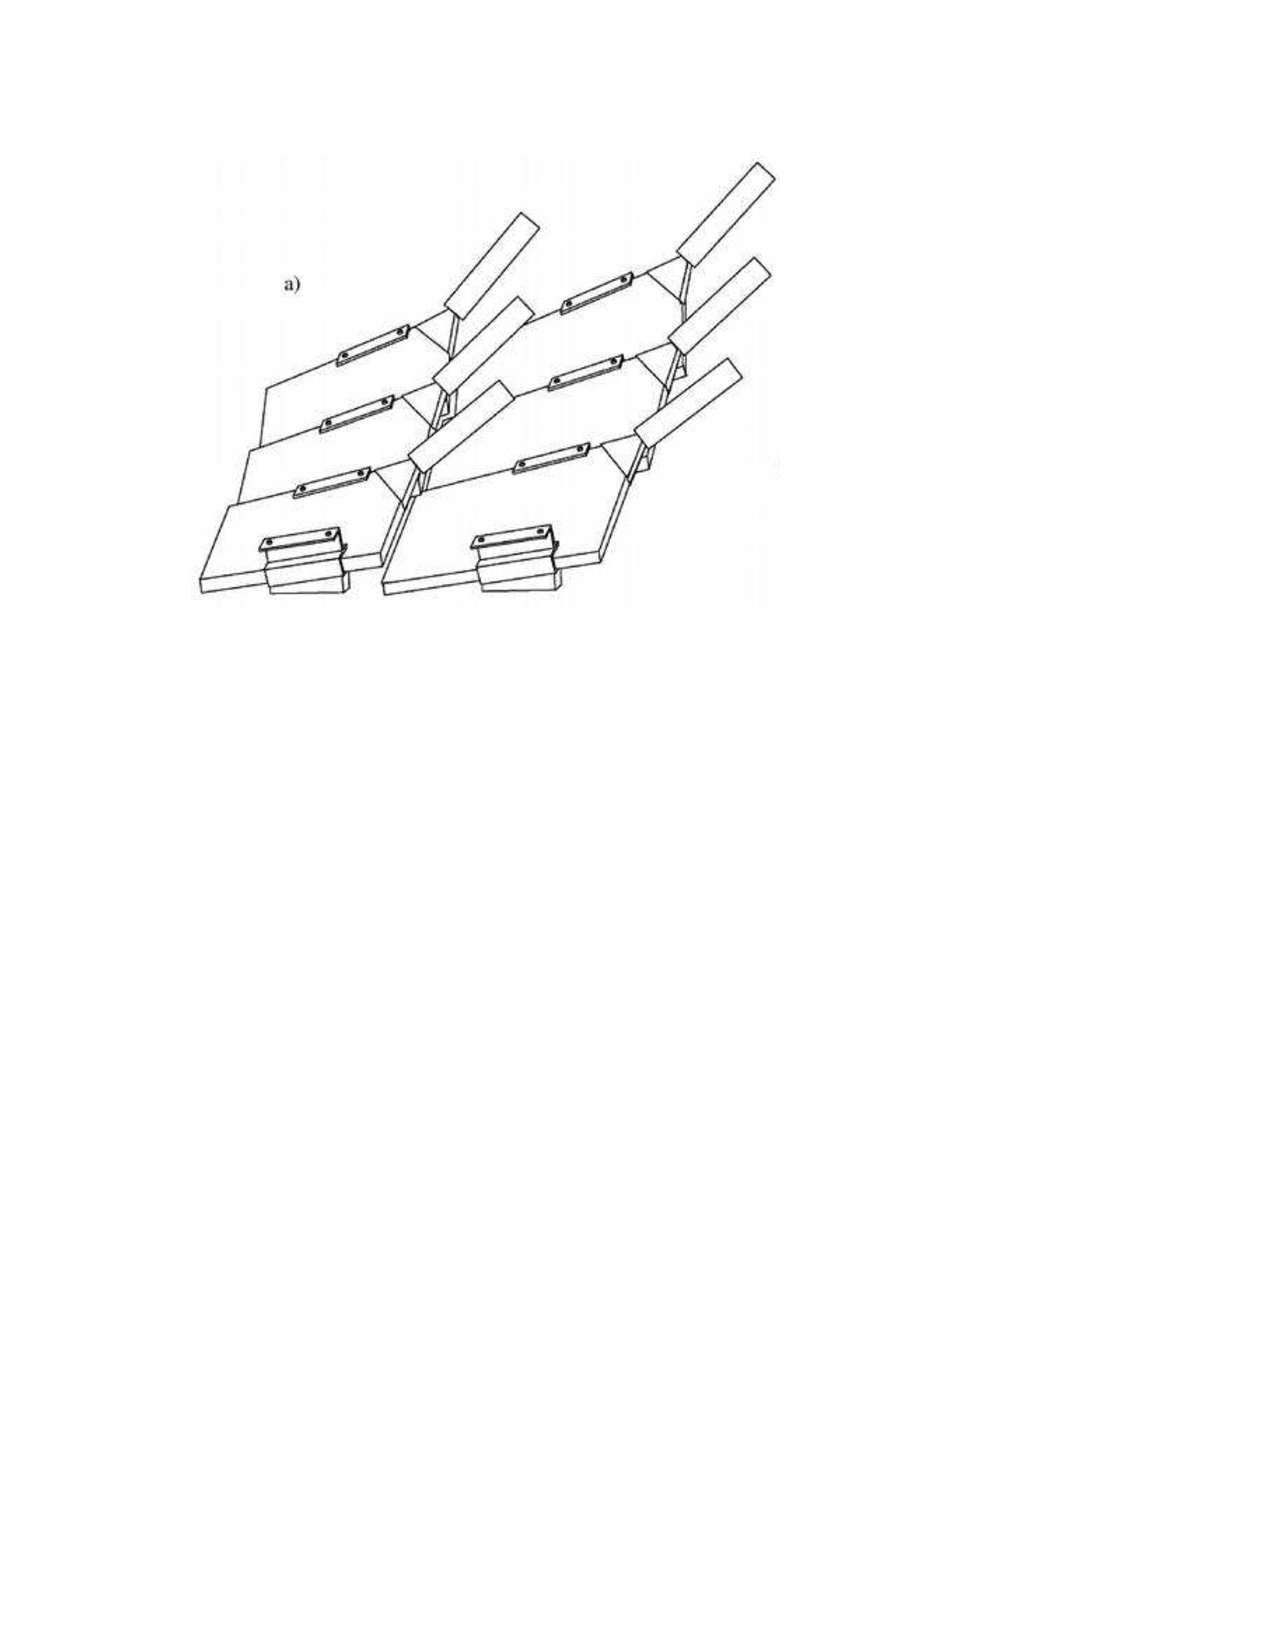
\includegraphics[height=0.45\textheight]{./Images/47_MD_forward_pixels_03.pdf}
      \caption*{Left: The design of a pixel scintillation counter.
        Right: counters arrangement}
    \end{figure}
    
  \end{overlayarea}
\end{frame}


%%%%%% SLIDE
\begin{frame}{\textcolor{Goldenrod}{Muon Forward Scintillation
      Counters Performance}}
  \begin{overlayarea}{\textwidth}{\textheight}
    \begin{figure}[h]
      \centering
      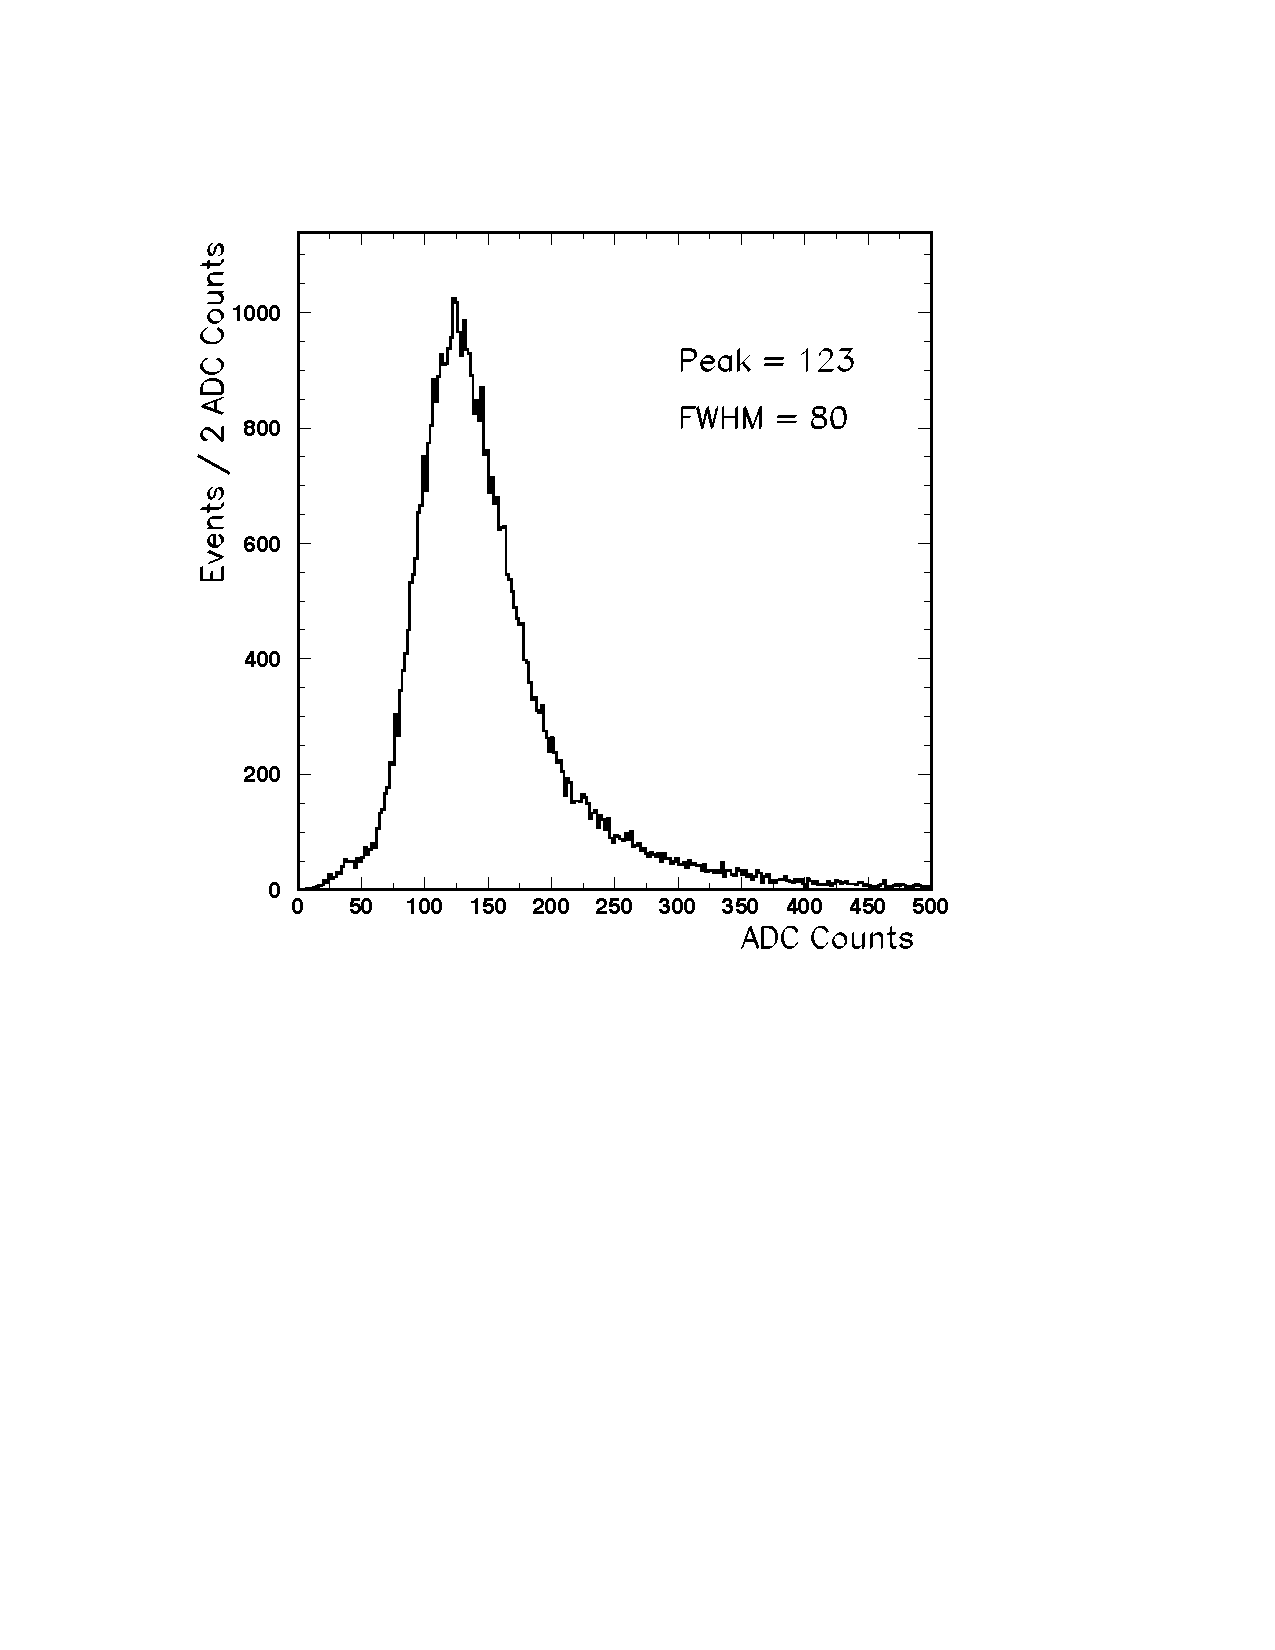
\includegraphics[width=0.25\textwidth]{./Images/47_MD_forward_pixels_05.pdf}\\
      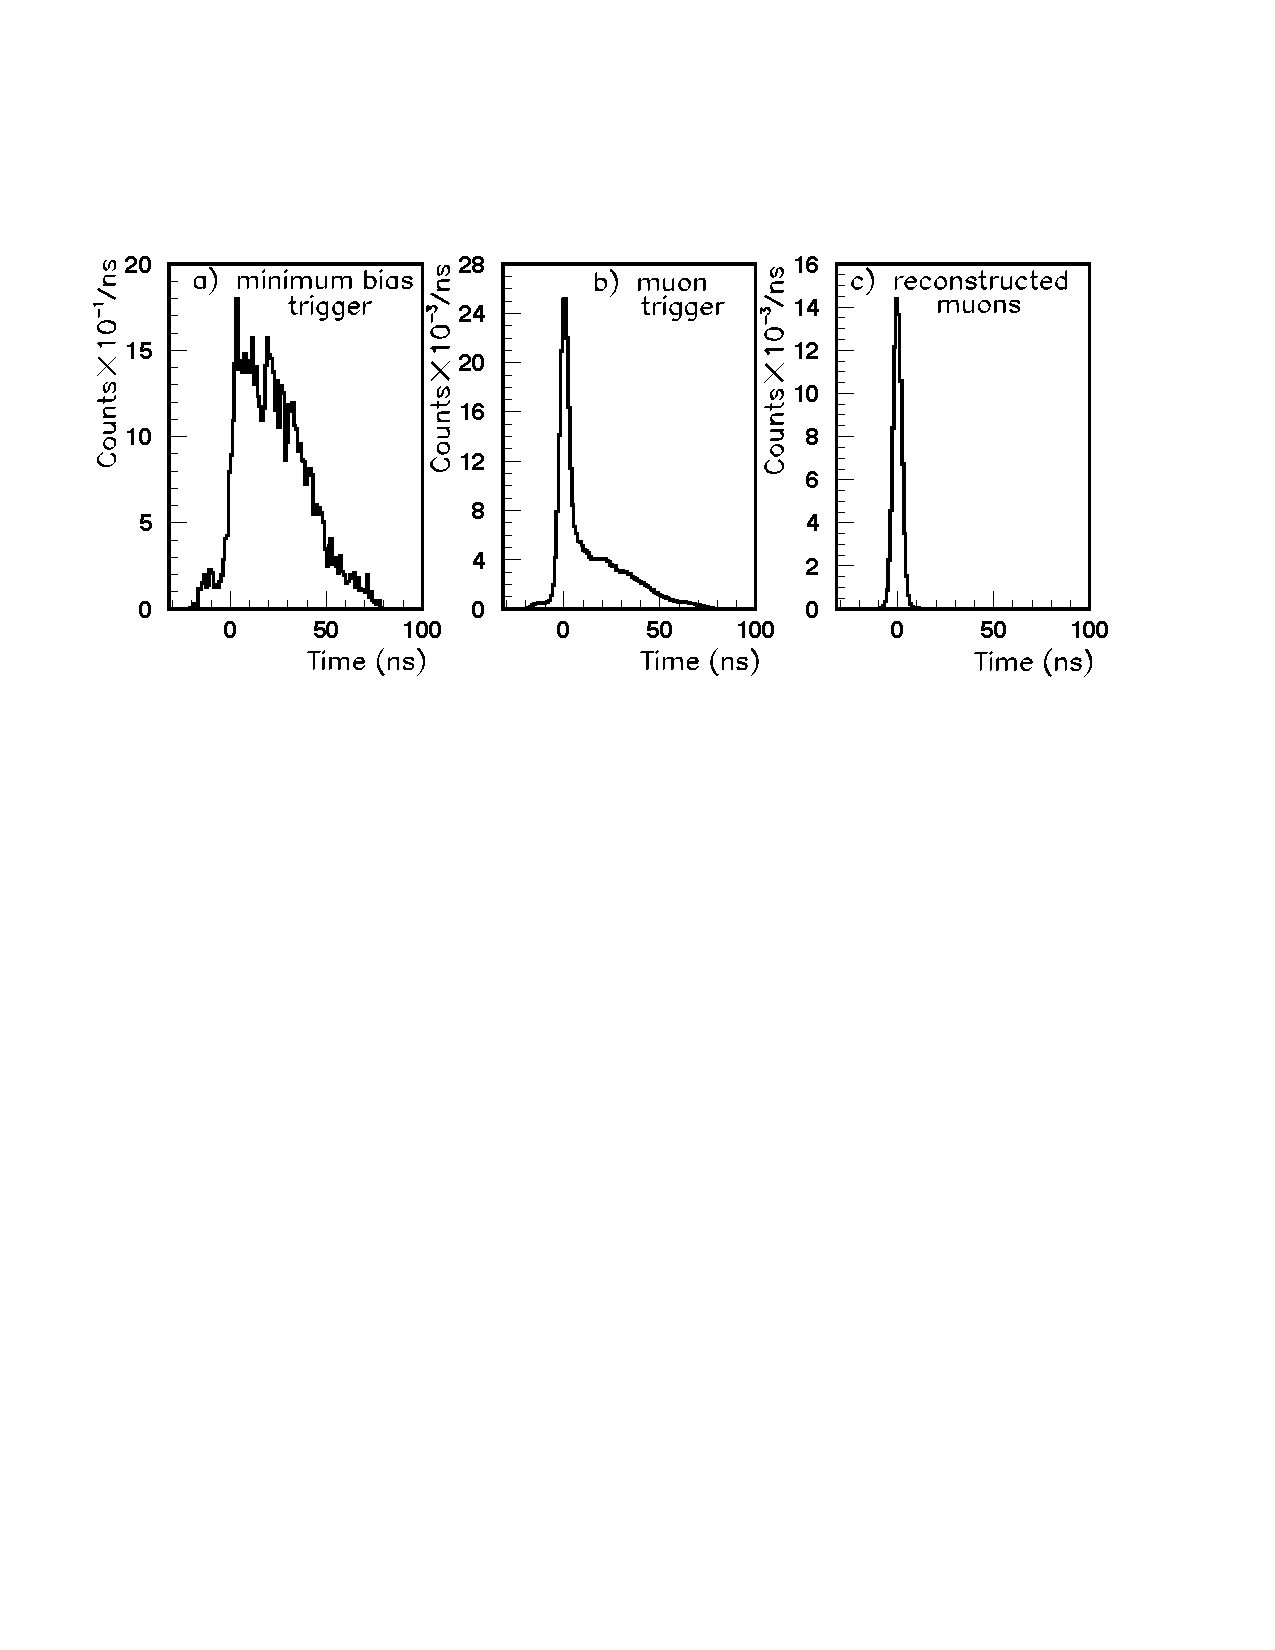
\includegraphics[width=0.75\textwidth]{./Images/47_MD_forward_pixels_06.pdf}
      \caption*{{\scriptsize Top: Muon pulse height distribution for all 4214 pixel
        counters. Bottom: Time spectra of hits recorded by pixel
        counters: a) minimum bias trigger; b) muon trigger; c)
        reconstructed muons.}}
    \end{figure}
  \end{overlayarea}
\end{frame}


